\documentclass[11pt, a4paper]{article}		% general format


%%%% Charset
\usepackage[utf8]{inputenc}					% use utf8					
\usepackage[russian]{babel}					% use russian font


%%%% Math
\usepackage{amsmath}						% Amer­i­can Math­e­mat­i­cal So­ci­ety (AMS) math fa­cil­i­ties
\usepackage{amsfonts}						% fonts from the AMS
\usepackage{amssymb}						% additional math symbols


%%%% Graphics
\usepackage{graphicx}


\author{Дедков Сергей}
\title{Отчет по лабораторной работе №1 :\\ \LaTeX{}, Git, GPG}
\date{2015}

%---------------------------------------------------------

\begin{document}
\maketitle
\tableofcontents
\newpage

%---------------------------------------------------------

\section{Cистема верстки \TeX{} и расширения \LaTeX{}}

%---------------------------------------------------------

\subsection{Цель работы}
Изучение принципов верстки \TeX{}, создание первого отчета

%---------------------------------------------------------

\subsection{Ход работы}

%---------------------------------------------------------

\subsubsection{Создание минимального файла .tex в простом текстовом редакторе – преамбула, тело документа}
Структура самого простого документа \LaTeX{} выглядит следующим образом:

\begin{verbatim}
	\documentclass{article}
	\usepackage[utf8]{inputenc}
	\usepackage[russian]{babel}
	\begin{document}
	Hello!!
	\end{document}
\end{verbatim}

Создадим файл test.tex. И введем в него данный код.

После комипляции подобный документ выведет просто слово Hello!!

Рассмотрим подробнее структуру документа:

Документ делиться на две части: \textit{преамбула} и \textit{тело} документа.

\textit{Преамбула} - часть с которой начинется документ(с начала до \verb'\begin{document}'), в которой вы задаете класс документа, его классовые опции, параметры страницы, подключаете пакеты, которые собираетесь использовать при верстке. 
Так, каждый входной файл должен начинаться с команды 

\verb'\documentclass{...}'

Она указывает, документ какого типа вы собираетесь писать. После этого можно включать команды, влияющие на стиль документа в целом, или загружать пакеты, с новыми возможностями. Для загрузки такого пакета используется команда

\verb'\usepackage{...}'

Далее следует \textit{тело} документа - начинается с \verb'\begin{document}' и заканчивается \verb'\end{document}'. В тело документа пишеться текст документа.

%---------------------------------------------------------

\subsubsection{Компиляция в командной строке – latex, xdvi, pdflatex}
Скомпилируем файл test.tex в командной строке.

Для этого воспользуемся командой latex:

\verb'latex test.tex'

После компиляции в той же папке будет создан файл test.dvi.

DVI (от англ. DeVice Independent — аппаратно независимый) — формат выходных файлов издательской системы.
Далее .dvi файлы преобразуются в другие читабельные форматы.

Преобразовать его можно, например, в pdf, используя комманду dvipdfm.

Чтобы создать pdf файл сразу из tex файла можно воспользоваться коммандой pdflatex.

%---------------------------------------------------------

\subsubsection{Оболочка TexMaker, Быстрый старт, Быстрая сборка}

Texmaker это кросс-платформенный open source \LaTeX{} редатктор с интегрриованной программой для просмотра PDF-файлов, написанный на Qt.
Оболочка TexMaker удобна в использованиии включает в себя множество настроек.

Texmaker с помощью функции Быстрый старт позволяет сформировать преамбулу документа, используя GUI.
Ниже на рисунке представлени образец формы Быстрый старт.

\begin{figure}[h!]
\centering
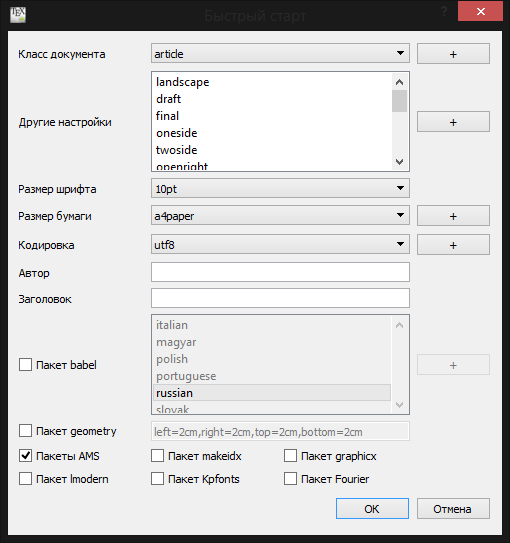
\includegraphics[scale=0.68]{res/fast_start}
\caption{Окно Быстрый старт}
\end{figure}

Самый простой способ скомпилировать документ — это использовать команду "Быстрая сборка". Задать последовательность команд используемых командой "Быстрый старт" можно в диалоге "Настроить Texmaker". Для запуска команды из панели инструментов сначала выберем ее, а затем нажмем кнопку "Run".

\begin{figure}[h!]
\centering
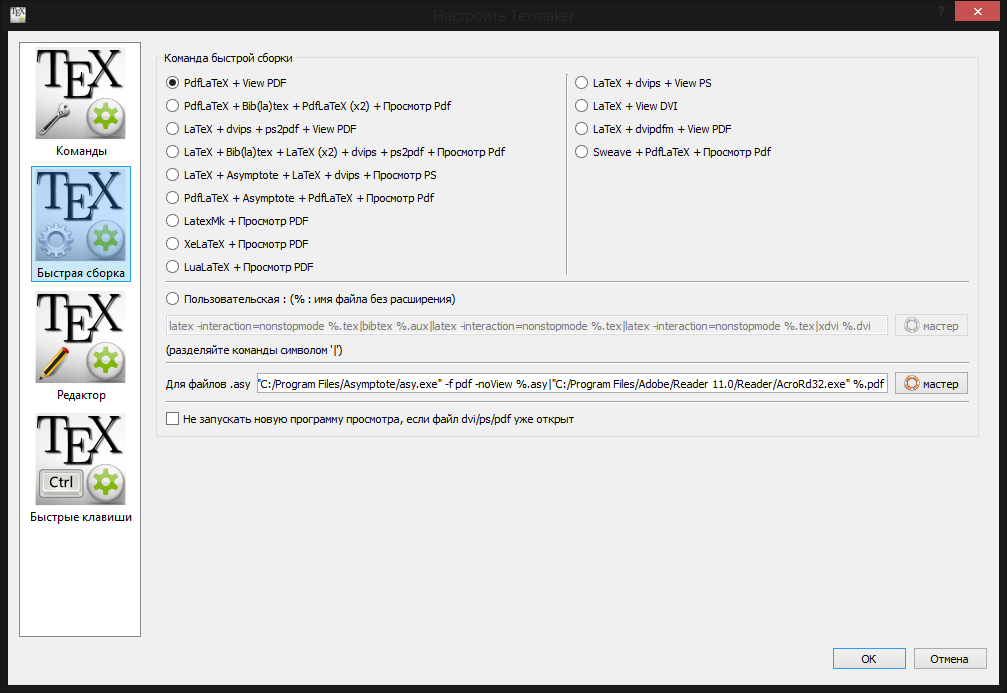
\includegraphics[scale=0.50]{res/fast_build}
\caption{Окно Быстрый старт}
\end{figure}

%---------------------------------------------------------

\subsubsection{Создание титульного листа, нескольких разделов, списка, несложной формулы}

Для создания титульного листа в преамбулу документа следует добавть следующие команду \verb'\title{...}'. Так же опционально можно указать автора и дату: \verb'\author{...}', \verb'\date{...}'. Пример:

\begin{verbatim}
	\author{Jane Smith}
	\title{My article}
	\date{2015}
\end{verbatim}

Чтобы титульный лист отобразился нужно уже в теле документа указать команду: \verb'\maketitle{...}'. Так же можно указать команду разрава страницы, чтобы титульный лист отбразился на отдельной странице \verb'\newpage{...}'.
\\Пример документа с титульным листом:
\begin{verbatim}
	\documentclass{article}
	\usepackage[utf8]{inputenc}
	\usepackage[russian]{babel}
	
	\author{Jane Smith}
	\title{My article}
	\date{2015}
	\begin{document}
	\maketitle
	\newpage
	
	Hello!!
	\end{document}
\end{verbatim}

Для создания разделов используются команды \verb'\section{...}', \verb'\subsection{...}', \verb'\subsubsection{...}' (секция, подсекция, под-подсекция соответсвенно). Следует отметить, что их следует использовать в правильном порядке.
\\Для выделения параграфов используются команды: \verb'\paragraph{...}' и \verb'\subparagraph{...}'
\\При разбиении документа на разделы есть возможность автоматического создания оглавления с помощью команды \verb'\maketitle'.

Окружение \verb'itemize' подходит для создания простых списков, окружение \verb'enumerate' - для нумерованых, а окружение \verb'descrioption' - для описаний.
\\Пример:
\begin{verbatim}
	\flushleft
	\begin{enumerate}
	\item Вы можете как угодно смешивать окружения списков: 
	\begin{itemize}
	\item Но это может смотреться глупо.
	\item[-] С минусом.
	\end{itemize}
	\item Поэтому помните:
	\begin{description}
	\item[Глупые] вещи не станут умнее от помещения в список.
	\item[Умные] вещи, однако, вполне можно представить списком.
	\end{description}
	\end{enumerate}
\end{verbatim}

Для отображения математических формул применяются следующие конструкции:
\begin{itemize}
\item \verb'$...$' - для формул внутри тектса. Результат: $a^2+b^2=c^2$
\item \verb'\[...\]' - для формул текст которых следует начать по центру в новой строке. Результат: \[a^2+b^2=c^2\]
\end{itemize}

%---------------------------------------------------------

\subsubsection{Понятие классов документов, подключение пакетов}

Как было отмечено выше в документе существует служебная часть, называемая преамбулой. В этой части указывается помимо прочего класс документа и подключаемые пакеты. Класс определяет тип документа, пакеты расширяют возможности \LaTeX{}.

Классы документов:
\begin{itemize}
\item \textbf{article} - статьи в журналах, краткие отчеты, презентации, приглашения...
\item \textbf{report} - для больших длинных отчетов, содержащих несколько глав, небольших книг, диссертаций...
\item \textbf{book} - для книг.
\item \textbf{slides} - для слайдов. Использует большие буквы без засечек. Вместо этого можно использовать Foil\TeX{}.
\end{itemize}

Пакет активизируются командой \verb'\usepackage'[\textit{опции}]{\textit{пакет}.
\textit{Пакет} - имя пакета. \textit{Опции} - список ключевых слов, включающий специальные свойства пакета.
Некоторые пакеты включены в основню поставку, другие предоставляются отдельно.

%---------------------------------------------------------

\subsubsection{Верстка более сложных формул}

Существует возможность задавать различные стили оформления форм:
Мы уже попробовали создать простую включенную и выключенную формулы. Теперь создадим что-то более сложное. Для ясного задания стиля оформления формул используются четыре команды:
\begin{itemize}
\newcommand{\ud}{\mathrm{d}}
\item Выключенная формула - \verb'$\dispalystyle': $ \int\!\!\!\int_{D} g(x,y) \, \ud x\, \ud y $
\item Текстовая формула - \verb'$\textstyle': $\textstyle \int\!\!\!\int_{D} g(x,y) \, \ud x\, \ud y$
\item Индексная формула - \verb'$\scriptstyle': $\scriptstyle \int\!\!\!\int_{D} g(x,y) \, \ud x\, \ud y$
\item Подиндексная формула - \verb'$\sciptscriptstyle': $\scriptscriptstyle \int\!\!\!\int_{D} g(x,y) \, \ud x\, \ud y$
\end{itemize}

Для написания тех или иных формул существуют соответствующие команды. Их достаточно много, поэтому не имеет смысл все перечислять. Достаточно воспользоваться справочным пособием при написании формул и найти там необходимые команды. Пример нескольких сложных формул ниже:

\begin{itemize}
\item Предел: 
	\begin{displaymath}
	\lim_{x \rightarrow 0} \frac{\sin x}{x}=1
	\end{displaymath} 
\item Матрица:
	\begin{displaymath}
	\mathbf{X} = \left( \begin{array}{ccc}
	x_{11} & x_{12} & \ldots \\
	x_{21} & x_{22} & \ldots \\
	\vdots & \vdots & \ddots
	\end{array} \right)
	\end{displaymath}
\item Оператор суммы: 
	\begin{displaymath}
	\sum_{\substack{0<i<n \\ 1<j<m}} P(i,j)
	\end{displaymath}
\end{itemize}


%---------------------------------------------------------

\subsection{Выводы}
\LaTeX{} - очень удобный инструмент. В освоении может сначала показаться сложным, но после кратковременного использования начинает нравиться.
Плюсом того, что верстка задается в коде является возможность одновременного редактирования несколькими людьми один документ, после чего совмещать изменения используя системы контроля версий.

%---------------------------------------------------------

\section{Система контроля версий Git}

%---------------------------------------------------------

\subsection{Цель работы}
Изучить систему контроля версий Git, освоить основные приемы работы с ней.


%---------------------------------------------------------

\subsection{Ход работы}

%---------------------------------------------------------

\subsubsection{Изучить справку для основных комманд}
Основные команды которые следует знать: init, clone, status, commit, pull, push, switch, checkout, branch.
Ресусрс для ознакомления https://git-scm.com/ - здесь можно найти примеры применения этих команд, а так же пошагово научиться работать с СКВ git.
Ниже будут рассмотрены случаи применения этих команд.


%---------------------------------------------------------

\subsubsection{Получить содержимое репозитория}
Для получения содержимого репозитория используется команда \verb'clone'.

Синтаксис: \verb'git clone <repository>'

\verb'<repository>' - URL к репозиторию, он может быть как локальный, так и через сеть интернет.

Ниже привеодиться пример получения содержимого репозитория github.

%---------------------------------------------------------

\subsubsection{Добавление новой папки и первого файла под контроль версий}
Для начала отметим, что пустые папки не добавляются под контроль версий, контролируются только файлы.

После создания папки и внутри нее файла система контроля версий автоматически начинает контролировать этот файл, если только в файле .gitignore не прописано иного. Как формруется файл .gitignore можно найти на просторах сети интернет, воспользовавшись, например, поисковой системой google.

Теперь, если после добавления не совершалось никаких действий, в частности, если пользователь не вызывал команду commit.

Посмотреть добавленные файлы можно воспользовавшись командой status.


%---------------------------------------------------------

\subsubsection{Зафиксировать изменения в локальном репозитории}
Чтобы зафиксировать изменения в локальном репозитории(тот что у пользователя на компьютере, пока что не внося изменений в удаленный репозиторий), следует воспользоваться командами:

\begin{itemize}
\item git add - для добавления файла в текущую ревизию. Это нужно для того, чтобы, например, не вносить всех изменений за одну ревизию, а резделить на этапы. Сначала добавить одни файлы, затем другие. В рамках этого примера добавляются все файлы.
\item git cimmit - фиксация изменений в ревизии, в локальном репозитории.
\end{itemize}

%---------------------------------------------------------

\subsubsection{Внести изменения в файл и просмотреть различия}
Если теперь изменть файл и воспользоваться после этого командой git status, измененный файл будет помечен, как modified.

Для просмотрa конкретных изменений существет команда:
\verb'git diff'

%---------------------------------------------------------

\subsubsection{Отменить локальные изменения}
Может случиться, так, что сделанные изменения не устраивают пользователя и ему хотелось бы вернуть файл или несколько файлов к исходному состоянию.

Для этого существует команда:
\verb'git checkout -- <filename>'


%---------------------------------------------------------

\subsubsection{Зафиксировать изменения в локальном репозитории, зафиксировать изменения в центральном репозитории}
Для фиксации изменений необходимо вызвать команду. git commit -a -m "commit message".

В центральном репозитории изменения фиксируются командой git push.


%---------------------------------------------------------

\subsubsection{Получить изменения из центрального репозитория}
Получение изменений из центрального репозитория - git pull.


%---------------------------------------------------------

\subsubsection{Поэкспериментировать с ветками}
Создание ветки - git checkout -b.

Переключение веток - git checkout.

Совмещение изменений в ветках - git merge.


%---------------------------------------------------------

\subsection{Выводы}
Система контролья версий git позволяет осуществлять командную разработку. Удобная в использовании и легкая в освоении. Так же можно использовать помимо командной строки - программы, которые предоставляют пользовательский интерфейс.


%---------------------------------------------------------

\section{Программа для шифрования и подписи GPG, пакет Gpg4win}

%---------------------------------------------------------

\subsection{Цель работы}

Научиться создавать сертификаты, шифровать файлы и ставить ЭЦП.


%---------------------------------------------------------

\subsection{Ход работы}

%---------------------------------------------------------

\subsubsection{Изучить документацию, запустить графическую оболочку Kleopatra}

В ходе выполнения лабораторной работы была установлена и освоена графическая оболочка Kleopatra.

%---------------------------------------------------------

\subsubsection{Создать ключевую пару OpenPGP (File->New Certificate)}

Была создана ключевая пара OpenPGP (PGP/MIME). Для этого в главном меню выбираем File->New Certificate. Далее из предложенных вариантов указываем, что необходимо создать ключевую пару OpenPGP. После этого вводим имя, электронную почту и passphrase. Далее ждем пока будет создана пара ключей Open PGP и нажимаем Finish.


%---------------------------------------------------------

\subsubsection{Экспортировать сертификат (File->Export Certificate)}

Эскортируем сертификат выбрав в главном меню File->Export Certificate и указав папку, куда необходимо произвести экспорт. В этой папке будет создан файл с расширением .asc, который содержит открытый ключ. Теперь этот файл можно передать партнеру, для возможности передавать сообщения и файлы в зашифрованном виде.

%---------------------------------------------------------

\subsubsection{Поставить ЭЦП на файл (File->Sing/Encrypt Files)}

Что бы подписать файл выберем в главном меню пункт File->Sing /Encrypt Files. Теперь укажем файл, который необходимо подписать и выберем пункт Sing. Указываем сертификат, которым производится подпись и файла. Теперь подтверждаем выбор и нажимаем Sing. Вводим passphrase в диалоговом окне PIN-кода. После того, как подпись будет создана, появится файл подписи с расширением .sig.


%---------------------------------------------------------

\subsubsection{Получить чужой сертификат из репозитория, файл с данными и файл с сигнатурой(подписью)}

Из репозитория возьмем файл с данными - myfirst.pdf, файл подписи - myfirst.pdf.sig и файл сертификата - karina.asc.

%---------------------------------------------------------

\subsubsection{Импортировать сертификат, подписать его}

Для импортирования сертификата в главном меню выбираем File->Import Certificates и выберем в качестве сертификата файл karina.asc. После чего сертификат будет добавлен в список импортированных сертификатов.

%---------------------------------------------------------

\subsubsection{Проверить подпись}

Для проверки подлинности и целостности файла myfirst.pdf нажмем на нем правой кнопкой, выберем пункт контекстного меню: Другие параметры GpgEX->Проверить. Для проверки целостности и подлинности необходимо, чтобы файл подписи лежал в одной папке с исходным файлом. Это позволит автоматически найти соответствие между ними. Подтвердим операцию нажатием Decrypt/Check. В случае успеха, будет выдано соответствующее сообщение. Если же в файле было произведено малейшее изменение, после совершение подписи, то подтверждение целостности пройдет неудачно.

%---------------------------------------------------------

\subsubsection{Взять сертификат кого-либо из коллег, зашифровать и подписать для него какой-либо текст, предоставить свой сертификат, убедится, что ему удалось получить открытый текст, проверить подпись.}

Для пары ключей OpenPGP возможно одновременно подписать и зашифровать файл. Причем подпись происходит до шифрования, что позволяет проверить подлинность и целостность файла только после расшифровки. Для этого в главном меню выбираем пункт File->Sing/Encrypt Files, указываем путь до файла, а далее указываем пункт Sing end Encrypt. После этого указываем все сертификаты, которыми будет шифровать файл и производим подпись и шифрование. Будет создан файл с расширением .gpg. Эксперимент был проведен в паре с моим коллегой, Николаем Патраковым. Мною был зашифрован и подписан документ Privet.docx, приложенный к отчету. В итоге получился файл Privet.docx.gpg, они был отправлен Николаю. Как сообщил мой коллега, эксперимент прошел успешно и файл был им расшифрован и прочитан.

%---------------------------------------------------------

\subsubsection{Предыдущий пункт наоборот}

Мной был взят файл с открытым ключом и импортирован в систему Kleopatra. Далее получив файл 111.txt.gpg от Николая, расшифровал и проверил подпись. Эксперимент прошел успешно. Содержимое файла: Привет). Файл приложен к отчету.


%---------------------------------------------------------

\subsubsection{Изучить GNU Privacy handbook, протестировать в использовании gpg через интерфейс командной строки, без использования графических оболочек.}

Были изучены следующие команды:

\begin{itemize}
\item --gen-key – создание новой пары ключей. Команда –edit-key позволяет в последствии изменить параметры ключа.
\item --sign – создает подпись для указанных файлов, используя ключ (если не введен его идентификатор, использует ключ по-умолчанию). --detach-sign создаст подпись в отдельном файле, иначе создается совмещенная подпись.
\item --encrypt – указывает на то, что данные надо зашифровать. Если применяется совместно с –-sign то данные одновременно подписываются.
\item --symmetric – можно применять когда просто надо зашифровать файл (используется симметричный алгоритм, но можно выбрать алгоритм командой --cipher-algo).
\item --decrypt – расшифровывает указанные файлы и сохраняет результат в файл (если указан) или выводит в консоль. Если файлы содержат подпись, она также проверяется.
\item --verify – проверяет подписи для указанных файлов, не выводя содержимого файла.
\item --list-keys – выводит список всех открытых ключей. Команда --list-secret-keys показывает ваши секретные ключи.
\item --delete-key – удаляет открытый ключ из списка. --delete-secret-key удаляет секретный ключ (например, он скомпрометирован или окончился срок действия)
\item --export (--import) – экспорт/импорт ваших ключей, например, для резервирования или переноса на другой компьютер. По умолчанию ключи в бинарном виде, для получения их в ASCI-виде укажите параметр –armor.
\end{itemize}

%---------------------------------------------------------

\subsection{Выводы}
В ходе выполнения третьего пункта лабораторной работы была освоена программа Kleopatra, входящая в пакет Gpg4win и используемая для шифрования и подписи GPG. Была создана пара ключей OpenGPG, в которой закрытый ключ защищен при помощи passphrase, а открытый ключ распространяется как сертификат(файл с расширением .asc). Произведен импорт нескольких сертификатов, что позволило зашифровать файлы, которые могут быть расшифрованы только владельцами этих сертификатов. Также была произведена подпись документов и соответственно проверка целостности и подлинности этих и других документов. Для проверки целостности и подлинности файла необходим сам файл, а также файл подписи.


\end{document}